In this section we present the \posi\ task. \pos\ tags are pre-requisite for many text applications. The task of \pos\ tagging where one is given a labeled training set of words and respective tags is a well studied task with several methods achieving high prediction quality, as we saw in the first part of this chapter. %Chapters \ref{day:seq} and \ref{day:seq_disc}. 

On the other hand the task of \posi\ where one does not have access to a labeled corpus is a much harder task with a huge space for improvement. In this case, we are given only the raw text along with sentence boundaries and a predefined number of clusters we can use. This problem can be seen as a clustering problem. We want to cluster words that behave grammatically in the same way on the same cluster. This is a much harder problem.

%Formally, the problem setting is the following: we are given a training set $\X = \sent^1 \ldots \sent^D$ of $D$ training examples, where each example $\sent = \obs_1 \ldots \obs_N$ is a sentence of $N$ words, whose values $\vv$ are taken from a vocabulary $\vocab$ of possible word types. We are also given the set of clusters $\hvocab$ that we are allowed to use. The hidden structure $\hseq = \hs_1 \ldots \hs_N$ corresponds to a sequence of cluster assignments for each individual word, such that $\hs_n = \hv_l$ with $\hv_l \in \hvocab$. 
%
Depending on the task at hand we can pick an arbitrary number of clusters. If the goal is to test how well our method can recover the true POS tags then we should use the same number of clusters as POS tags. On the other hand, if the task is to extract features to be used by other methods we can use a much bigger number of clusters (e.g., 200) to capture correlations not captured by POS tags, like lexical affinity. 

Note, however that nothing is said about the identity of each cluster. The model has no preference in assigning cluster 1 to nouns vs cluster 2 to nouns. Given this non-identifiability several metrics have been proposed for evaluation \citep{Reichart09,haghighi2006naacl,Meila07,RosenbergH07}. In this class we will use a common and simple metric called \textbf{1-Many}, which maps each cluster to majority pos tag that it contains (see Figure \ref{fig:cm_uns} for an example). 

\begin{figure}[h!]
\centering
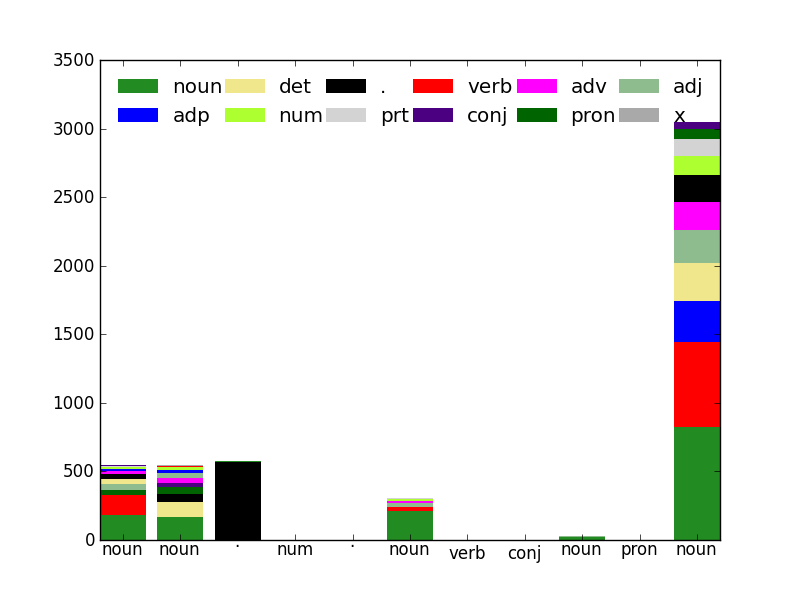
\includegraphics[scale=.5]{figs/sequences/cm_uns1.png}
\caption{\label{fig:cm_uns} Confusion Matrix example. Each cluster is a column. The best tag in each column is represented under the column (1-many) mapping. Each color represents a true Pos Tag.}
\end{figure}


\begin{exercise}
Run 20 epochs of the EM algorithm for part of speech induction:
\begin{python}
>>> hmm.train_EM(train_seq, 0.1, 20, evaluate=True)
>>> viterbi_pred_test = hmm.viterbi_decode_corpus(test_seq)
>>> posterior_pred_test = hmm.posterior_decode_corpus(test_seq)
>>> eval_viterbi_test =   hmm.evaluate_corpus(test_seq, viterbi_pred_test)
>>> eval_posterior_test = hmm.evaluate_corpus(test_seq, posterior_pred_test)

Initial accuracy: 0.303638
Iter: 1 Log Likelihood: -101824.763927
Iter: 1 Accuracy: 0.305441
Iter: 2 Log Likelihood: -78057.108346
Iter: 2 Accuracy: 0.321976
Iter: 3 Log Likelihood: -77813.725501
Iter: 3 Accuracy: 0.357451
Iter: 4 Log Likelihood: -77192.947674
Iter: 4 Accuracy: 0.385109
Iter: 5 Log Likelihood: -76191.800849
Iter: 5 Accuracy: 0.392123
Iter: 6 Log Likelihood: -75242.572729
Iter: 6 Accuracy: 0.391121
Iter: 7 Log Likelihood: -74392.892496
Iter: 7 Accuracy: 0.404249
Iter: 8 Log Likelihood: -73357.542833
Iter: 8 Accuracy: 0.399940
Iter: 9 Log Likelihood: -72135.182778
Iter: 9 Accuracy: 0.399238
Iter: 10 Log Likelihood: -70924.246230
Iter: 10 Accuracy: 0.395430
Iter: 11 Log Likelihood: -69906.561800
Iter: 11 Accuracy: 0.394328
Iter: 12 Log Likelihood: -69140.228623
Iter: 12 Accuracy: 0.390821
Iter: 13 Log Likelihood: -68541.416423
Iter: 13 Accuracy: 0.391522
Iter: 14 Log Likelihood: -68053.456865
Iter: 14 Accuracy: 0.389117
Iter: 15 Log Likelihood: -67667.318961
Iter: 15 Accuracy: 0.386411
Iter: 16 Log Likelihood: -67337.685686
Iter: 16 Accuracy: 0.385409
Iter: 17 Log Likelihood: -67054.571821
Iter: 17 Accuracy: 0.385409
Iter: 18 Log Likelihood: -66769.973881
Iter: 18 Accuracy: 0.385409
Iter: 19 Log Likelihood: -66442.608458
Iter: 19 Accuracy: 0.385409

>>> confusion_matrix = cm.build_confusion_matrix(test_seq.seq_list, viterbi_pred_test, 
                                             len(corpus.tag_dict), hmm.get_num_states())
>>> cm.plot_confusion_bar_graph(confusion_matrix, corpus.tag_dict, 
                            xrange(hmm.get_num_states()), 'Confusion matrix')
\end{python}
Note: your results may not be the same as in this example since we are using a random start, but the trend should be the same, 
with log-likelihood increasing at every iteration. 
%Also note that in some iterations the likelihood does not go down because of some rounding errors, however the general trend is that likelihood decreases over iterations. 
\end{exercise}

In the previous exercise we used an HMM to do Part-of-Speech induction using 12 clusters (by omission the HMM uses as number 
of hidden states the one provided by the corpus). A first observation is that the log-likelihood is always increasing as expected. 
Another observation is that the accuracy goes up from 32\% to 38\%. 
Note that normally you will run this algorithm for 200 iterations, we stopped earlier for time constraints. 
Another observation is that the accuracy is not monotonic increasing, this is because the likelihood is not a perfect proxy 
for the accuracy. In fact all that the likelihood is measuring are co-occurrences of words in the corpus; it has no idea of pos tags. 
The fact that we are improving derives from the fact that language is not random but follows some specific hidden patterns. 
In fact this patterns are what true pos-tags try to capture. A final observation is that the performance is really bad 
compared to the supervised scenario, so there is a lot of space for improvement. The actual state of the 
art is around 71\% for fully unsupervised~\citep{JoaoThesis,bergkirkpatrick2010naacl} and 80\% \citep{das-petrov:2011:ACL-HLT2011} 
using parallel data and information from labels in the other language. 

Looking at Figure \ref{fig:cm_uns}, it shows the confusion matrix for this particular example. 
A first observation is that most clusters are mapped to nouns, verbs or punctuation. 
This is a known fact since there are many more nouns and verbs than any other tags. Since maximum likelihood prefers probabilities 
to be uniform (imagine two parameters: in one setting both have value 0.5 so the likelihood will be 0.5*0.5 = 0.25, 
while in the other case one as 0.1 and 0.9 so the maximum likelihood is 0.09). Several approaches have been proposed to 
address this problem, moving towards a Bayesian setting \citep{johnson2007dtf}, or using 
Posterior Regularization \citep{graca2009nips}. 
%more about this later today. 
%Part-of-Speech induction is a very active field of research, in fact in the last two ACL conferences (Association for Computational Linguistics) the short paper award (2010) and the best paper award (2011) were about this topic~\citep{lamar-EtAl:2010:Short,das-petrov:2011:ACL-HLT2011}.








% \begin{exercise}

% Repeat the previous exercise using a different number of hidden states (20,50). Note that the higher the number of states is the slower the training will be.
% What do you observe? Look at the confusion matrix and try to explaing what is happening.

% \begin{python}
% In []: run readers/pos_corpus.py
% In []: posc = PostagCorpus("en",max_sent_len=15,train_sents=1000,dev_sents=0,test_sents=0)
% In []: run sequences/hmm.py
% In []: hmm = HMM(posc,nr_states=20)
% In []: hmm.initialize_radom()
% In []: run sequences/em.py
% In []: em = EM(posc,hmm)
% In []: em.train(posc.train,nr_iter=20)
% Init acc 0.348933
% Iter: 1 Negative Log Likelihood 16.038424
% Iter: 1 acc 0.362662
% Iter: 2 Negative Log Likelihood 11.200816
% Iter: 2 acc 0.370177
% Iter: 3 Negative Log Likelihood 11.046597
% Iter: 3 acc 0.380800
% Iter: 4 Negative Log Likelihood 10.607496
% Iter: 4 acc 0.389518
% Iter: 5 Negative Log Likelihood 9.809817
% Iter: 5 acc 0.394027
% Iter: 6 Negative Log Likelihood 8.949717
% Iter: 6 acc 0.396733
% Iter: 7 Negative Log Likelihood 8.105404
% Iter: 7 acc 0.398337
% Iter: 8 Negative Log Likelihood 7.366612
% Iter: 8 acc 0.392925
% Iter: 9 Negative Log Likelihood 7.005009
% Iter: 9 acc 0.393126
% Iter: 10 Negative Log Likelihood 6.895723
% Iter: 10 acc 0.397034
% Iter: 11 Negative Log Likelihood 6.851836
% Iter: 11 acc 0.397134
% Iter: 12 Negative Log Likelihood 6.818365
% Iter: 12 acc 0.399238
% Iter: 13 Negative Log Likelihood 6.782213
% Iter: 13 acc 0.406053
% Iter: 14 Negative Log Likelihood 6.755121
% Iter: 15 Negative Log Likelihood 6.745873
% Iter: 15 acc 0.419681
% Iter: 16 Negative Log Likelihood 6.743681
% Iter: 16 acc 0.424291
% Iter: 17 Negative Log Likelihood 6.745030
% Iter: 17 acc 0.431406
% Iter: 18 Negative Log Likelihood 6.747628
% Iter: 18 acc 0.434512
% Iter: 19 Negative Log Likelihood 6.749084
% Iter: 19 acc 0.438721
% pred = hmm.viterbi_decode_corpus(posc.train.seq_list)
% cm = build_confusion_matrix(posc.train.seq_list,pred,len(posc.int_to_pos),hmm.nr_states)
% plot_confusion_bar_graph(cm,posc.int_to_pos,range(12),"test")
% \end{python}

% \end{exercise}

%%% Local Variables: 
%%% mode: latex
%%% TeX-master: "../../guide"
%%% End: 
